\chapter{Prosody}\label{chap:prosody}

This chapter is not for beginners. You may skip this in the first reading. Just going through it roughly, however, has its own merit. You will know what we can do about the subject with this powerful tool.

Pāli prosody, or \pali{chanda}, is a big, difficult topic to learn. I am not keen on this subject, nor I am a poetry enthusiast. I see it from an engineering point of view that if we have a good tool we can learn this hard topic easier, or even with fun. There are several things to learn before you can use this tool effectively. When it is first opened, it shows just a list of prosodic types. When you click on a row, you just see a bizarre formula at the bottom border (see Figure \ref{fig:prosody-first}).\footnote{For the full list of prosodic patterns, see Appendix \ref{chap:prospatt}.}

\begin{figure}[!hbt]
\centering
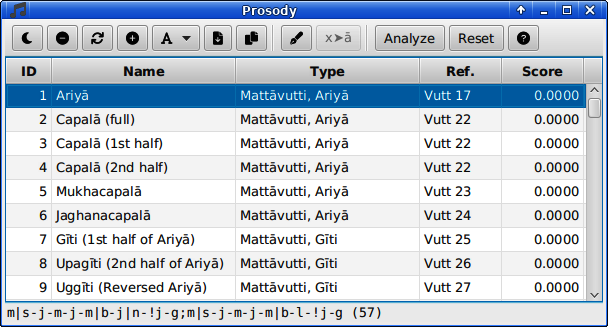
\includegraphics[width=0.9\linewidth]{images/prosody-first.png}\\
\caption{Prosody window}
\label{fig:prosody-first}
\end{figure}

For I have never mentioned Pāli prosody in my previous books, I will do it in this chapter just enough to understand how the program works. The main, in fact only, work that we refer to is \emph{Vuttodaya}.\footnote{The author is Saṅgharakkhita of Udumbaragiri, around the 12th-13th century AD, in Sri Lanka. This book is included in the collection of traditional grammar books. The text is so terse that we can make little sense out of it. Fortunately, I have Vuttodayamañjarī by Gandhasārābhivaṃsa, printed by Mahachulalongkorn Buddhist University, Nakhon Pathom, Thailand (2001). This commentary on Vuttodaya is written in Thai. It is comprehensive and well-organized. I think this is what a commentary should be. Writing new commentaries with modern languages is preferable nowadays because we can make them very clear to the readers, as exemplified by this work. If you cannot read them, certainly someone can, and now AI probably can too. Writing a new text with Pāli makes things worse, and does little help to the textual understanding. For English readers, I find a translation by Ānandajoti Bhikkhu useful, but not beginner-friendly, see \url{www.ancient-buddhist-texts.net/Textual-Studies/Vuttodaya/index.htm}.}

\section{A survival introduction to Pāli prosody}

As a subject, prosody is ``The study of the metrical structure of verse.''\footnote{The American Heritage Dictionary, \url{www.ahdictionary.com/word/search.html?q=prosody}} For our concern, it is the way to put words into an organized structure ruled by groups of syllables. At the fundamental level, a Pāli syllable can be either `light' (\pali{lahu}) or `heavy' (\pali{garu}). To measure this `weight' we consider only vowels in a word.

\paragraph{\pali{Lahu} is short open vowels.} When \pali{a, i,} or \pali{u} sits by itself alone or follows a consonant, and \textbf{not} followed by a double-consonant or \pali{ṃ}, it is counted as `light.' \pali{Lahu} weighs 1 unit (measure). So, we use symbol \texttt{\bfseries 1} and \texttt{\bfseries l} here.\footnote{Many textbooks on the subject use \smallsmile\ for \pali{lahu} and -- for \pali{garu}, or vice versa (see Vutt\,7). I find this very confusing, so I avoid using these symbols.} 

\paragraph{\pali{Garu} is everything else.} When you can identify \pali{lahu}, \pali{garu} is simply the rest of that. \pali{Garu} weighs 2 units. We use symbol \texttt{\bfseries 2} and \texttt{\bfseries g} here.\footnote{The symbol \texttt{\bfseries 2} has double meaning. It means \pali{garu} in an analyzed result (as we shall see shortly). And if the symbol appears in a formula, it means any combination that give 2 measures long, i.e., both ll (1+1) and g (2) can be counted as 2. This may make some confused, but I insist on using 1 and 2 because they look better and clearer.}

\boxnote{Remember that:\\
\hspace{5mm}\bullet\ \pali{lahu} is short vowels, not followed by a double-consonant or \pali{ṃ}, other things else are \pali{garu}.\\
\hspace{5mm}\bullet\ \texttt{\bfseries 1} only means \pali{lahu}.\\
\hspace{5mm}\bullet\ \texttt{\bfseries 2} is context dependent, meaning \pali{garu} in an analyzed result, and two \pali{lahu}s or one \pali{garu} in the formulas.
}

\bigskip
Let us see an example to make sure we get the same picture. In fact, I make a tool that can calculate the meter of any text. It is a part of the program's Text Editor. A result of meter calculation is shown in Figure \ref{fig:editor-meter}. For more information, see Chapter \ref{chap:editor}.

\begin{figure}[!hbt]
\centering
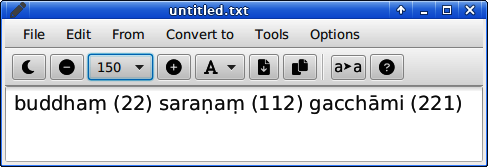
\includegraphics[width=0.7\linewidth]{images/editor-meter.png}\\
\caption{Meter calculation in the program's Editor}
\label{fig:editor-meter}
\end{figure}

In the result, \pali{lahu} and \pali{garu} are denoted by \texttt{1} and \texttt{2} respectively. First, \pali{buddhaṃ} gets \texttt{22} because the \pali{u} is followed by \pali{ddh} (double consonants), and the \pali{a} is followed by \pali{ṃ}. Second, \pali{saraṇaṃ} gets \texttt{112} because the first two \pali{a} are open short vowels, whereas the last one is followed by \pali{ṃ}. And third, \pali{gacchāmi} gets \texttt{221} because the \pali{a} is followed by \pali{cch} (double consonants), the \pali{ā} is a long vowel, and the \pali{i} is an open short vowel.\footnote{Some may wonder ``What about a short vowel followed by a single consonant (which does not belong to the next syllable)?'' Put it bluntly, there is no such a thing. You may see \pali{tad} here and there in Pāli books, but not in the traditional textbooks. We will never see \pali{tad} stands alone. It is \pali{taṃ} with \pali{d} substitution as a result of word-joining (\pali{Sandhi}). So, that syllable may be either of \pali{lahu} or \pali{garu} type depending on whether the \pali{d} is doubled or not.}

Now we can see that when we put words together by a constraint of \pali{lahu-garu} patterns, we are composing a verse. The whole business of Pāli prosody is to recognize patterns and to put words into patterns.

\section{Two types of prosodic patterns}

Broadly speaking, there are two ways to put syllables into pattern: (1) by counting the syllables, and (2) by counting the weight or measure. Understanding the distinction between the two is crucial, so let make it clear first. We can illustrate the two types of counting by using the example above in Table \ref{tab:metersum-example}.

\begin{table}[!hbt]
\centering
\caption{Syllable vs.\ weight summation}
\label{tab:metersum-example}
\bigskip
\begin{tabular}{>{\itshape}llcc} \toprule
\upshape\bfseries Word & \bfseries Meter & \bfseries Syllable sum & \bfseries Weight sum \\ \midrule
buddhaṃ & 22 & 2 & 4 \\
saraṇaṃ & 112 & 3 & 4 \\
gacchāmi & 221 & 3 & 5 \\
\bottomrule
\end{tabular}
\end{table}

By those ways of counting, \emph{Vuttodaya} categorizes prosodic patterns into two, namely \pali{mattāvutti} and \pali{vaññavutti}. The former uses weight-counting, mainly with 4-measure groups (\pali{gaṇa}). The latter uses syllable-counting, mainly with 3-syllable groups. Table \ref{tab:mattagroup} summarizes the \pali{mattāvutti} groups used in the program's prosodic formulas, whereas Table \ref{tab:vannagroup} summarizes the \pali{vaññavutti} groups.

\boxnote{Two types of prosodic patterns are as follows:\\
\hspace{5mm}\bullet\ \pali{Mattāvutti}, counting the weight or measures of words\\
\hspace{5mm}\bullet\ \pali{Vaññavutti}, counting the syllables of words
}

\setcounter{table}{1}
\begin{table}[!hbt]
\centering
\caption{Meter groups used in \pali{mattāvutti}}
\label{tab:mattagroup}
\bigskip
\begin{tabular}{>{\ttfamily}c>{\ttfamily}cl} \toprule
\rmfamily\bfseries Symbol & \rmfamily\bfseries Group & \bfseries Notes \\ \midrule
n & 1111 & \pali{Na gaṇa} \\
s & 112 & \pali{Sa gaṇa} \\
j & 121 & \pali{Ja gaṇa} \\
b & 211 & \pali{Bha gaṇa} \\
m & 22 & \pali{Ma gaṇa} \\
4 & any & any of the above five \\
6 & any & any of the above five plus \texttt{g} or \texttt{ll} \\
8 & any & any combination of the above five \\
l & 1 & \pali{lahu} \\
g & 2 & \pali{garu} \\
2 & any & \texttt{g (2)} or \texttt{ll (11)} \\
\bottomrule
\end{tabular}
\end{table}

In the tables, we can see that in \pali{mattāvutti} there are 5 main groups (\pali{gaṇa}), all have 4-unit weight but variable syllables. The names of \pali{gaṇa} are traditional, but I use lowercase here to distinguish them from \pali{vaññavutti} types. In the latter case, there are 8 main groups, all have 3 syllables but variable weight. Some names are common, some are new. Note carefully on \pali{Na gaṇa} and \pali{Ma gaṇa}, which share the name but not the content. I use uppercase in the latter. The 14-\pali{lahu} group (\texttt{L}) is used only in the program, not in any textbooks. Some of \pali{mattāvutti} verse types use the symbols of \pali{vaññavutti} in their formula. For example, Vetālīya (Vutt\,29) uses \texttt{R} (212), Opacchandasaka (Vutt\,30) uses \texttt{R} and \texttt{Y} (122), and Acaladhiti (Vutt\,38) uses \texttt{L}.\footnote{To make it clear, using symbols in the formulas has nothing to do with the tradition. It is a convenient way for computation in programming.}

\begin{table}[!hbt]
\centering
\caption{Meter groups used in \pali{vaññavutti}}
\label{tab:vannagroup}
\bigskip
\begin{tabular}{>{\ttfamily}c>{\ttfamily}cl} \toprule
\rmfamily\bfseries Symbol & \rmfamily\bfseries Group & \bfseries Notes \\ \midrule
N & 111 & \pali{Na gaṇa} \\
S & 112 & \pali{Sa gaṇa} \\
J & 121 & \pali{Ja gaṇa} \\
Y & 122 & \pali{Ya gaṇa} \\
B & 211 & \pali{Bha gaṇa} \\
R & 212 & \pali{Ra gaṇa} \\
T & 221 & \pali{Ta gaṇa} \\
M & 222 & \pali{Ma gaṇa} \\
l & 1 & \pali{lahu} \\
g & 2 & \pali{garu} \\
L & 14 \times\ l & used only in the program \\
\bottomrule
\end{tabular}
\end{table}

As described above, it is possible that one passage can be analyzed by both methods, resulting in different patterns. Let us see the analysis of our example above in Table \ref{tab:metersum-example-grouped}. There are many possibilities how to put syllables into a group even when using the same method, as shown in the table.\footnote{8/13 = syllable sum/weight sum} This variety gives us a number of predefined patterns presented in \pali{Vuttodaya}, as we shall see in the next sections.

\begin{table}[!hbt]
\centering
\caption{Syllable vs.\ weight grouping}
\label{tab:metersum-example-grouped}
\bigskip
\begin{tabular}{ll} \toprule
Passage & \pali{buddhaṃ saraṇaṃ gacchāmi} \\
Raw meter & \texttt{22 112 221 (8/13)} \\
Mattāvutti grouping 1 & \texttt{22-112-22-1 = m-s-m-l} \\
Mattāvutti grouping 2 & \texttt{2-211-22-21 = g-b-m-gl} \\
Vaññavutti grouping 1 & \texttt{22-112-221 \ = gg-S-T} \\
Vaññavutti grouping 2 & \texttt{221-122-21 \ = T-Y-gl} \\
\bottomrule
\end{tabular}
\end{table}

Before we are going to see the verse list, let me explain some symbols used in verse formulas. I translated the descriptive rules into computable formulas. So, they look weird to non-programmer users. But the formulas are not difficult to read if you try to understand the symbols. Beside of meter-group symbols described above, there are also special symbols, as shown in Table \ref{tab:formula-symbols}.

\begin{table}[!hbt]
\centering
\caption{Symbols in verse formulas}
\label{tab:formula-symbols}
\bigskip
\begin{tabular}{ll} \toprule
\bfseries Symbol & \bfseries Meaning \\ \midrule
Vertical bar (\texttt{|}) & logical OR \\
Exclamation mark (\texttt{!}) & logical NOT \\
Semicolon (\texttt{;}) & line separator \\
Hyphen (\texttt{-}) & mere separator \\
\bottomrule
\end{tabular}
\end{table}

We will see how logical OR and NOT work when I put a real formula into explanation. The line separator (\texttt{;}), if present, tells us that the pattern needs 2 lines of verse to make the analysis complete. If the input passage is not long enough, or does not have 2 lines as required, `\texttt{incomplete}' will be shown in the status bar. But, if the analyzed text has more syllables than the formula requires, `\texttt{over-required}' will be shown instead. Hyphen (\texttt{-}) is just a separator, having no meaning. It only makes formulas easier to read.

\section{Verse types of \pali{mattāvutti}}

\pali{Vuttodaya} starts with definitions and general rules, then verse types of \pali{mattāvutti} are listed. We can divide further into 4 subgroups, namely, Ariyā, Gīti, Vetālīya, and Mattāsamaka. All verse types (\pali{gāthā}) in each subgroup are listed in Table \ref{tab:mattaverses}. Not all of these can be analyzed by the program, as noted below.

\bigskip
\begin{longtable}[c]{p{0.05\linewidth}p{0.40\linewidth}p{0.05\linewidth}p{0.23\linewidth}p{0.1\linewidth}}
\caption{Verse types of \pali{mattāvutti}}\label{tab:mattaverses}\\
\toprule
\bfseries ID & \bfseries Name & \bfseries WS\footnotemark & \bfseries \mbox{Parent group} & \bfseries Ref. \\ \midrule
\endfirsthead
\multicolumn{5}{c}{\tablename\ \thetable: Verse types of \pali{mattāvutti} (contd\ldots)}\\
\toprule
\bfseries ID & \bfseries Name & \bfseries WS & \bfseries \mbox{Parent group} & \bfseries Ref. \\ \midrule
\endhead
\bottomrule
\ltblcontinuedbreak{5}
\endfoot
\bottomrule
\endlastfoot
%
\footnotetext{Weight Sum, the total weight required}
1 & Ariyā & 57 & Ariyā & Vutt\,17 \\
-- & Paṭhayā & 57 & Ariyā & Vutt\,20 \\
-- & Vipulā & 57 & Ariyā & Vutt\,21 \\
2 & Capalā (full) & 57 & Ariyā & Vutt\,22 \\
3 & Capalā (1st half) & 30 & Ariyā & Vutt\,22 \\
4 & Capalā (2nd half) & 27 & Ariyā & Vutt\,22 \\
5 & Mukhacapalā & 57 & Ariyā & Vutt\,23 \\
6 & Jaghanacapalā & 57 & Ariyā & Vutt\,24 \\
7 & Gīti (1st half of Ariyā) & 30 & Gīti & Vutt\,25 \\
8 & \mbox{Upagīti (2nd half of Ariyā)} & 27 & Gīti & Vutt\,26 \\
9 & Uggīti (Reversed Ariyā) & 57 & Gīti & Vutt\,27 \\
10 & Ariyāgīti & 32 & Gīti & Vutt\,28 \\
11 & Vetālīya & 30 & Vetālīya & Vutt\,29 \\
12 & Opacchandasaka & 34 & Vetālīya & Vutt\,30 \\
13 & Āpātalikā & 30 & Vetālīya & Vutt\,31 \\
14 & Dakkhiṇantikā & 30 & Vetālīya & Vutt\,32 \\
15 & Udiccavutti & 30 & Vetālīya & Vutt\,33 \\
16 & Paccavutti & 30 & Vetālīya & Vutt\,34 \\
17 & Pavattaka & 30 & Vetālīya & Vutt\,35 \\
18 & Aparantikā (1) & 32 & Vetālīya & Vutt\,36 \\
19 & Aparantikā (2) & 32 & Vetālīya & Vutt\,36 \\
20 & Cāruhāsinī (1) & 28 & Vetālīya & Vutt\,37 \\
21 & Cāruhāsinī (2) & 28 & Vetālīya & Vutt\,37 \\
22 & Acaladhiti & 16 & Mattāsamaka & Vutt\,38 \\
23 & Mattāsamaka & 16 & Mattāsamaka & Vutt\,39 \\
24 & Visiloka & 16 & Mattāsamaka & Vutt\,40 \\
25 & Vānavāsikā & 16 & Mattāsamaka & Vutt\,41 \\
26 & Citrā & 16 & Mattāsamaka & Vutt\,42 \\
27 & Upacitrā & 16 & Mattāsamaka & Vutt\,43 \\
-- & Pādākulaka & 16 & Mattāsamaka & Vutt\,44 \\
\end{longtable}

Verse types in this category have complicated formulas. So, let us go slowly. Normally, one stanza consists of 4 feet (quarter, \pali{pāda}) or 2 lines. Some verse types need 2-line pattern, some need only 1-line to complete the analysis. This sounds a bit tricky. Normally, we do not compose a single-line verse. At least, we need two lines. However, many patterns have repeated formula for the first and second line. As a result, checking only one line for such patterns is enough. A suggestion here is ``Always analyze two lines of verse.'' Let us see the metrical pattern of Ariyā:

\bigskip
\begin{tabular}{>{\large\ttfamily}*{2}l}
!j-4-!j-4-!j-j|n-!j-g; & (30) \\
!j-4-!j-4-!j-l-!j-g & (27) \\
\end{tabular}
\bigskip

The pattern needs 2 lines (see \texttt{;}). The first line is read \texttt{NOT j, 4, NOT j, 4, NOT j, j OR n, NOT j, g}. The second is read \texttt{NOT j, 4, NOT j, 4, NOT j, l, NOT j, g}. As shown in Table \ref{tab:mattagroup}, \texttt{4} means any of meter groups is applicable, \texttt{NOT j} means any meter group but \texttt{j}, and \texttt{j OR n} means either \texttt{j} or \texttt{n} is valid.

Let us see a real example. This stanza is the first one of Ganthārambhakathā in Dīghanikāya-aṭṭhakathā.

\begin{quote}
{\small\pali{Karuṇāsītalahadayaṃ, paññāpajjotavihatamohatamaṃ;}}\\
\texttt{112-211-112, 22-22-1111-211-2;} \\
\texttt{s-b-s, m-m-n-b-g;} \\
{\small\pali{Sanarāmaralokagaruṃ, vande sugataṃ gativimuttaṃ.}}\\
\texttt{112-112-112, 22 112 1-112-2.}\\
\texttt{s-s-s, m s l-s-g.}\\
\end{quote}

If you carefully analyze the verse as shown above, you will see that it conforms to the pattern described perfectly. To analyze the verse by the program, first open the text mentioned by TOC Tree (see Chapter \ref{chap:browsing}), select the stanza and copy. Then open Prosody window and hit \texttt{Analyze} button. The most relevant results will show at the top of the table. The analyzed result against Ariyā pattern is shown in Figure \ref{fig:prosody-ariya}.

\begin{figure}[!hbt]
\centering
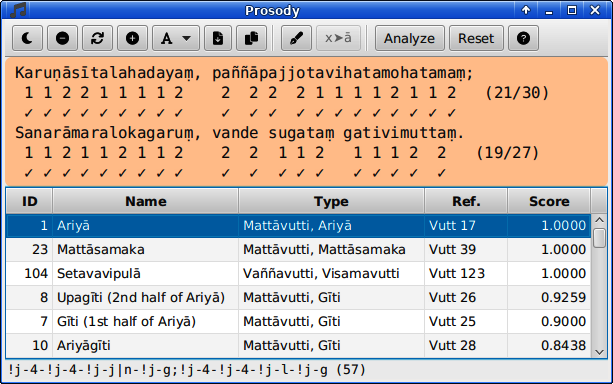
\includegraphics[width=0.9\linewidth]{images/prosody-ariya.png}\\
\caption{Analysis of \pali{Ariyā} verse type}
\label{fig:prosody-ariya}
\end{figure}

In the result table produced by the program, \emph{Score} is the calculation of percentage of matching between the text and the formula. So, \texttt{1.0} means 100\% matched. There are possibilities that we get multiple \texttt{1.0} results. But all of them are not always `correct' answers. Some portion of text may be totally matched against the formula, but the text is \texttt{over-required} as shown in Figure \ref{fig:prosody-over-required}.

Another noteworthy point, even though a result is not 100\% matched, it can be a correct answer. Most frequent cases are the unmatched last syllable of each line: it can be \texttt{g} despite the required \texttt{l}, or vice versa. And as you may find out yourselves later, exactly matched verses in the real text are quite rare, except newly composed ones that are crafted in that way. The real old verses are recalcitrant to the rules somehow. That is why many exceptions are mentioned in detailed textbooks on prosody.\footnote{An attempt to shoehorn a verse into a recognized pattern creates exceptions, or extra considerations, to the rules. I do not use that approach in the program. We just find the closest candidates and regard the verse as it is. I think this is the normal way how poetry is composed. To achieve certain artistic result, breaking some rules seems natural. Of course, there can be cases of half-baked poetry that just ignores or plays with rules. And, finally, there can be many cases that rules are held so firmly that the meter trumps the clarity of the words used---words are oddly changed to conform with rules.}

\begin{figure}[!hbt]
\centering
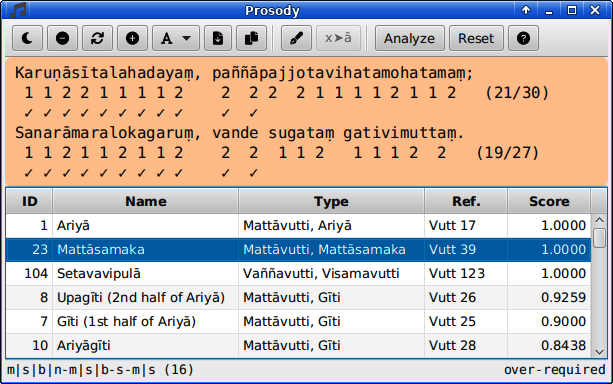
\includegraphics[width=0.9\linewidth]{images/prosody-over-required.png}\\
\caption{Example of an \texttt{over-required} case}
\label{fig:prosody-over-required}
\end{figure}

Now you can see how the program is really helpful in metrical analysis. Doing it by hand is tedious, laborious, and error-prone. Computer has its limitation, however. There are certain things unable to be analyzed, at least in a simple way, by the program. Metrical pause (caesura), or \pali{yati} in Pāli, is one of those.

Generally, metrical pause has two kinds. First, the pause after each foot ends. This is common in recitation and writing. When you read a verse, you are supposed to pause at points to make a sense of rhythm. And it is natural to pause at the end of a foot, probably a small pause after the odd feet, a bigger one after the first line (first even foot), and the biggest one after the second line (last even foot).

The second kind of pause is rarer, the pause inside the feet. Some verse types have rules about pauses, particularly the Ariyā group. Pauses at the endings is easy to see because punctuation marks can be used in text. But in-between pauses cannot be shown in the program, because this kind of pause makes sense only when the verse is recited.\footnote{The rules concerning metrical pause are not easy to understand, so I skip the explanation.}

Another limitation is the program cannot detect the spilled-over effect: a word is cut into two and both parts are split across feet. This aspect differentiates Vipulā (having a spilled-over) from Paṭhayā (no spilled-over).\footnote{From Vutt\,21, ``\pali{Yattha gaṇattaya mullaṅ-ghi, Yo'bhayatthā'dimo bhave vipulā.}'' According to the formula, the word \pali{mullaṅghi} has to be split so that the \pali{-ghi} part belongs to the latter foot.} As a result, the program can not tell the two verse types apart. They are grouped together under Ariyā.\footnote{There is also a confusion of this. According to the text, in Vutt\,19 Ariyāsāmañña is mentioned, and Paṭhayā is mentioned in Vutt\,20, Vipulā in Vutt\,21. So, it is supposed that Ariyāsāmañña and Paṭhayā are different kinds. But it is not very clear how they differ to each other. In a way, we can interpret that they are the same. By this concern, I drop Ariyāsāmañña from the list.}

It should be noted that Vetālīya (Vutt\,29) has a particular rule: ``No successive 6 \pali{lahu}s are allowed in the even feet.'' This means in its formula, \texttt{6-R-l-g-8-R-l-g}, the \texttt{8} in the second part does not allow neither \texttt{1111112} nor \texttt{2111111}. This rule has been already implemented.

Finally in this category, Pādākulaka (Vutt\,44) is an arbitrary combination of Mattāsamaka group. It has no fixed pattern to detect, so it is left out from analysis (no ID).\footnote{ID numbers used here have nothing to do with \pali{Vuttodaya}. They are used internally in the program. The users can use the numbers for sorting the table, by clicking the column header. To refer to a particular verse type, using a reference to \pali{Vuttodaya}, if any, is more reliable.}

\section{Verse types of \pali{vaññavutti}}

There are 3 main subgroups in this category: Samavutti (symmetry), Aḍḍhasamavutti (semi-symmetry), and Visamavutti (asymmetry). The sense of `symmetry' here means whether each foot (quarter) of a verse is equal in length. It can be that all 4 feet are equal (symmetry), or odd feet and even feet are equal (semi-symmetry), or arbitrary (asymmetry). All verse types in this category, plus some more, are listed in Table \ref{tab:vannaverses}.

In Vutt\,13, twenty-six types of (symmetric) prosody (\pali{chanda}) are mentioned. That is to say, in theory, the metrical patterns can run from 1 syllable to 26 syllables. \pali{Vuttodaya} itself, however, lists only seventeen types: from 6-syllable (Gāyattī) to 22-syllable (Ākati) pattern (see other names in footnotes).

\bigskip
\begin{longtable}[c]{p{0.05\linewidth}p{0.36\linewidth}p{0.05\linewidth}p{0.24\linewidth}p{0.1\linewidth}}
\caption{Verse types of \pali{vaññavutti}}\label{tab:vannaverses}\\
\toprule
	\bfseries ID & \bfseries Name & \bfseries SS\footnotemark & \bfseries \mbox{Parent group} & \bfseries Ref. \\ \midrule
\endfirsthead
\multicolumn{5}{c}{\tablename\ \thetable: Verse types of \pali{vaññavutti} (contd\ldots)}\\
\toprule
	\bfseries ID & \bfseries Name & \bfseries SS & \bfseries \mbox{Parent group} & \bfseries Ref. \\ \midrule
\endhead
\bottomrule
\ltblcontinuedbreak{5}
\endfoot
\bottomrule
\endlastfoot
%
\footnotetext{Syllable Sum, the total syllables required}
28 & Tanumajjhā & 6\footnote{Gāyattī} & Samavutti & Vutt\,46 \\
29 & Kumāralalitā & 7\footnote{Uṇhikā} & Samavutti & Vutt\,47 \\
30 & Citrapadā & 8\footnote{Anuṭṭhubhā} & Samavutti & Vutt\,48 \\
31 & Vijjummālā & 8 & Samavutti & Vutt\,49 \\
32 & Māṇavaka & 8 & Samavutti & Vutt\,50 \\
33 & Samānikā & 8 & Samavutti & Vutt\,51 \\
34 & Pamāṇikā & 8 & Samavutti & Vutt\,52 \\
35 & Halamukhī & 9\footnote{Barahatī} & Samavutti & Vutt\,53 \\
36 & Bhujagasususaṭā & 9 & Samavutti & Vutt\,54 \\
37 & Suddhavirājita & 10\footnote{Panti} & Samavutti & Vutt\,55 \\
38 & Paṇava & 10 & Samavutti & Vutt\,56 \\
39 & Rummavatī & 10 & Samavutti & Vutt\,57 \\
40 & Mattā & 10 & Samavutti & Vutt\,58 \\
41 & Campakamālā & 10 & Samavutti & Vutt\,59 \\
42 & Manoramā & 10 & Samavutti & Vutt\,60 \\
43 & Ubbhāsaka & 10 & Samavutti & Vutt\,61 \\
44 & Upaṭṭhitā & 10 & Samavutti & Vutt\,62 \\
45 & Indavajira & 11\footnote{Tiṭṭhubhā} & Samavutti & Vutt\,63 \\
46 & Upendavajira & 11 & Samavutti & Vutt\,64 \\
-- & Upajāti & 11 & Samavutti & Vutt\,65 \\
47 & Sumukhī & 11 & Samavutti & Vutt\,66 \\
48 & Dodhaka & 11 & Samavutti & Vutt\,67 \\
49 & Sālinī & 11 & Samavutti & Vutt\,68 \\
50 & Vātommī & 11 & Samavutti & Vutt\,69 \\
51 & Sirī & 11 & Samavutti & Vutt\,70 \\
52 & Rathoddhatā & 11 & Samavutti & Vutt\,71 \\
53 & Svāgatā & 11 & Samavutti & Vutt\,72 \\
54 & Bhaddikā & 11 & Samavutti & Vutt\,73 \\
55 & Vaṃsaṭṭha & 12\footnote{Jagatī} & Samavutti & Vutt\,74 \\
56 & Indavaṃsā & 12 & Samavutti & Vutt\,75 \\
57 & Toṭaka & 12 & Samavutti & Vutt\,76 \\
58 & Dutavilambita & 12 & Samavutti & Vutt\,77 \\
59 & Puṭa & 12 & Samavutti & Vutt\,78 \\
60 & Kusumavicittā & 12 & Samavutti & Vutt\,79 \\
61 & Bhujaṅgappayāta & 12 & Samavutti & Vutt\,80 \\
62 & Piyaṃvadā & 12 & Samavutti & Vutt\,81 \\
63 & Lalitā & 12 & Samavutti & Vutt\,82 \\
64 & Pamitakkharā & 12 & Samavutti & Vutt\,83 \\
65 & Ujjalā & 12 & Samavutti & Vutt\,84 \\
66 & Vessadevī & 12 & Samavutti & Vutt\,85 \\
67 & Tāmarasa & 12 & Samavutti & Vutt\,86 \\
68 & Kamalā & 12 & Samavutti & Vutt\,87 \\
69 & Pahassiṇī & 13\footnote{Atijagatī} & Samavutti & Vutt\,88 \\
70 & Rucirā & 13 & Samavutti & Vutt\,89 \\
71 & Aparājitā & 14\footnote{Sakkarī} & Samavutti & Vutt\,90 \\
72 & Paharaṇakalikā & 14 & Samavutti & Vutt\,91 \\
73 & Vasantatilakā & 14 & Samavutti & Vutt\,92 \\
74 & Sasikalā & 15\footnote{Atisakkarī} & Samavutti & Vutt\,93 \\
75 & Maṇiguṇanikara & 15 & Samavutti & Vutt\,94 \\
76 & Mālinī & 15 & Samavutti & Vutt\,95 \\
77 & Pabhaddaka & 15 & Samavutti & Vutt\,96 \\
78 & Vāṇinī & 16\footnote{Aṭṭhi} & Samavutti & Vutt\,97 \\
79 & Sikharaṇī & 17\footnote{Accaṭṭhi} & Samavutti & Vutt\,98 \\
80 & Hariṇī & 17 & Samavutti & Vutt\,99 \\
81 & Mandakkantā & 17 & Samavutti & Vutt\,100 \\
82 & Kusumitalatā & 18\footnote{Dhiti} & Samavutti & Vutt\,101 \\
83 & Meghavipphujjitā & 19\footnote{Atidhiti} & Samavutti & Vutt\,102 \\
84 & Saddūlavikkīḷita & 19 & Samavutti & Vutt\,103 \\
85 & Vutta & 20\footnote{Kati} & Samavutti & Vutt\,104 \\
86 & Sandharā & 21\footnote{Pakati} & Samavutti & Vutt\,105 \\
87 & Bhaddaka & 22\footnote{Ākati} & Samavutti & Vutt\,106 \\
88 & Upacitta & 22 & Aḍḍhasamavutti & Vutt\,107 \\
89 & Dutamajjhā & 23 & Aḍḍhasamavutti & Vutt\,108 \\
90 & Vegavatī & 21 & Aḍḍhasamavutti & Vutt\,109 \\
91 & Bhaddavirāja & 21 & Aḍḍhasamavutti & Vutt\,110 \\
92 & Ketumatī & 21 & Aḍḍhasamavutti & Vutt\,111 \\
93 & Ākhyānakī & 22 & Aḍḍhasamavutti & Vutt\,112 \\
94 & Viparītākhyānakī & 22 & Aḍḍhasamavutti & Vutt\,113 \\
95 & Hariṇaplutā & 23 & Aḍḍhasamavutti & Vutt\,114 \\
96 & Aparavatta & 23 & Aḍḍhasamavutti & Vutt\,115 \\
97 & Pupphitaggā & 25 & Aḍḍhasamavutti & Vutt\,116 \\
98 & Yavamatī & 25 & Aḍḍhasamavutti & Vutt\,117 \\
99 & Vatta & 16 & Visamavutti & Vutt\,118 \\
100 & Pathyāvatta & 16 & Visamavutti & Vutt\,119 \\
101 & Vīparītapathyāvatta & 16 & Visamavutti & Vutt\,120 \\
102 & Capalāvatta & 16 & Visamavutti & Vutt\,121 \\
103 & Piṅgalavipulā & 16 & Visamavutti & Vutt\,122 \\
104 & Setavavipulā & 16 & Visamavutti & Vutt\,123 \\
105 & Bhakāravipulā & 16 & Visamavutti & Vutt\,124 \\
106 & \mbox{Pathamabhakāravipulā} & 32 & Visamavutti & Vutt\,124 \\
107 & Tatiyabhakāravipulā & 32 & Visamavutti & Vutt\,124 \\
108 & Rakāravipulā & 16 & Visamavutti & Vutt\,125 \\
109 & \mbox{Pathamarakāravipulā} & 32 & Visamavutti & Vutt\,125 \\
110 & Tatiyarakāravipulā & 32 & Visamavutti & Vutt\,125 \\
111 & Nakāravipulā & 16 & Visamavutti & Vutt\,126 \\
112 & \mbox{Pathamanakāravipulā} & 32 & Visamavutti & Vutt\,126 \\
113 & Tatiyanakāravipulā & 32 & Visamavutti & Vutt\,126 \\
114 & Takāravipulā & 16 & Visamavutti & \\
115 & Pathamatakāravipulā & 32 & Visamavutti & \\
116 & Tatiyatakāravipulā & 32 & Visamavutti & \\
117 & Makāravipulā & 16 & Visamavutti & \\
118 & \mbox{Pathamamakāravipulā} & 32 & Visamavutti & \\
119 & Tatiyamakāravipulā & 32 & Visamavutti & \\
120 & Sakāravipulā & 16 & Visamavutti & \\
121 & \mbox{Pathamasakāravipulā} & 32 & Visamavutti & \\
122 & Tatiyasakāravipulā & 32 & Visamavutti & \\
123 & Jakāravipulā & 16 & Visamavutti & \\
124 & Pathamajakāravipulā & 32 & Visamavutti & \\
125 & Tatiyajakāravipulā & 32 & Visamavutti & \\
\end{longtable}

\pali{Vaññavutti} verse types are relatively easier to understand and analyze, but there is something to consider particularly about symmetric types. Formulas given in Samavutti are only for one foot, not one line or two feet (or full two lines or four feet) as we have seen in the other group. As a result, you have to edit the input passage by cutting one line of the verse into two, otherwise `\texttt{over-required}' will be the case. It is better to see a real example, as shown in Figure \ref{fig:prosody-tanumajjha}.

\begin{figure}[!hbt]
\centering
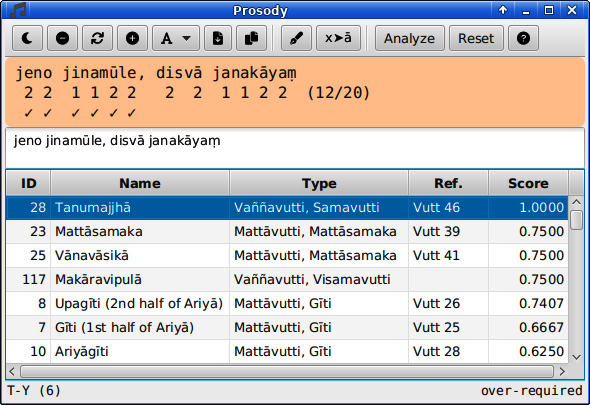
\includegraphics[width=0.9\linewidth]{images/prosody-tanumajjha-wrong.png}\\
(a) Over-required in full-line analysis\\[3mm]
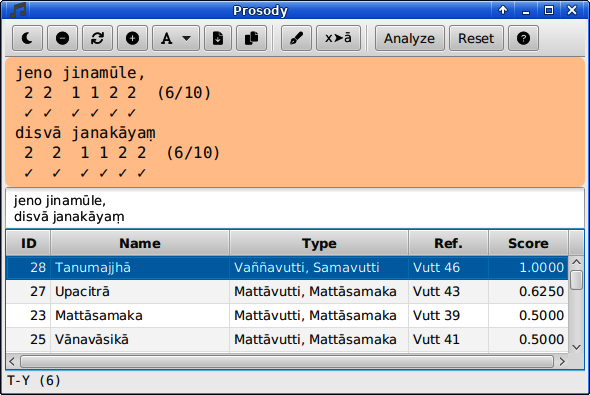
\includegraphics[width=0.9\linewidth]{images/prosody-tanumajjha-right.png}\\
(b) Correct result by a proper cut\\[4mm]
\caption{Analysis of \pali{Tanumajjhā} verse type}
\label{fig:prosody-tanumajjha}
\end{figure}

In the example, a line of Tanumajjhā (6-syllable \texttt{T-Y} pattern) type is shown.\footnote{The sample is taken from the 6th stanza of Mahāpaṇāmapāṭha, under Homage to the Buddha (Buddha-vandanā gantha-saṅgaho) in the Añña group of CST4 collection.} In the text, we have stanzas in full form. If you copy the whole line and analyze it, `\texttt{over-required}' will show. You have to cut the line by using edit mode ({\faSix \symbol{"F5AC}} button), then you will get the correct result. In semi-symmetry and asymmetry groups, the formulas are given for one whole line, so you do not have to do likewise in these groups.

There are some other notes the users should know. First, Upajāti (Vutt\,65) is a mixed-up of Indavajira (Vutt\,63) and Upendavajira (Vutt\,64), or sometimes from other types. So, it has no fixed pattern to detect, and it is left out from analysis (no ID).

Second, Sasikalā (Vutt\,93) and Maṇiguṇanikara (Vutt\,94) use the same formula (14 \pali{lahu}s plus 1 \pali{garu}) but the latter has two pauses, after the 8th syllable and the last one. These two are not distinguishable in the program, even though they are different.

And the last note, verse types ID 114 (Takāravipulā) to 125 (Tatiyajakāravipulā) have no references in \pali{Vuttodaya}. These types follow the logic of the previous Bhakāravipulā (Vutt\,124), Rakāravipulā (Vutt\,125), and Nakāravipulā (Vutt\,126).\footnote{These are added in Vuttodayamañjarī by Ven.\,Gandhasārābhivaṃsa.} I add them here because they are easy to implement the analysis.

There are other minor things I have not mentioned. The users should play around and find out how things work. Once you know this kind of tool exists, you can do research in Pāli prosody easier than before. For metrical composition, this tool can be your test bench. With the edit mode mentioned above, you can compose a short verse in real time. Furthermore, the program also provides \emph{search by meter} to help the users find a matched word to a pettern required. We will talk about this later in the related tool.
